\begin{frame}{Why faster machine learning?}

\vspace{0.05in}
\begin{tikzpicture}

%%%%%%%%%%%%%%%%%%%%%%%%%%%%%%%%%%%%%%%%

\node[text width=10cm] at (0,0) {
Facebook generates more than 200 terabytes of data per day (Facebook blog, 2014)
};

%\uncover<1>{
%\foreach \i in {1,...,20}
%\foreach \j in {1,...,10}
%{
    %\node at (0.5*\i-4.25,-2-0.5*\j) {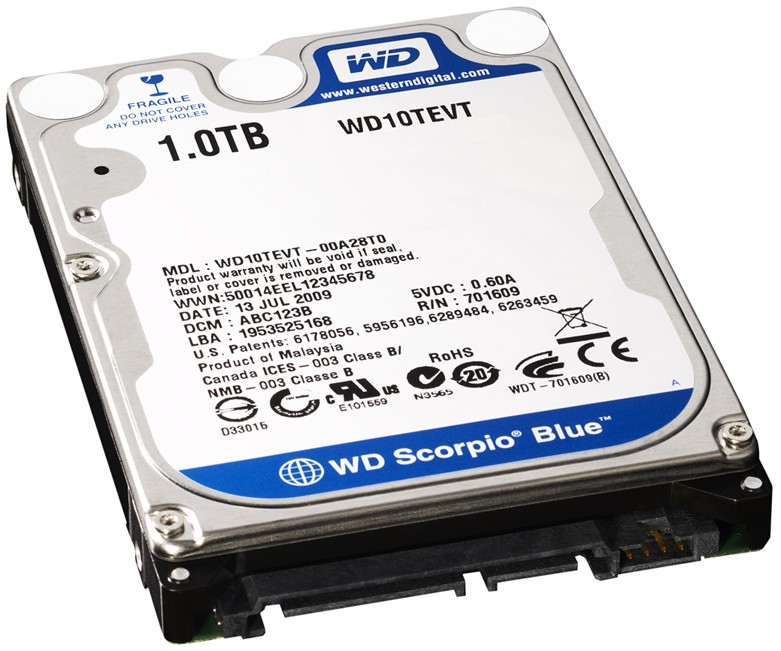
\includegraphics[width=0.4cm]{img-presentation/1tb}};
%}
%\node at (-4,-2) {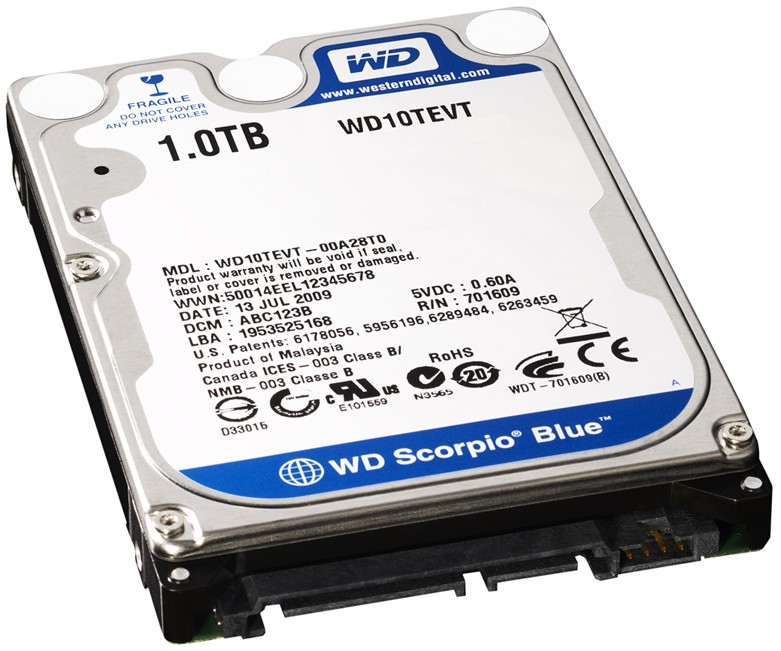
\includegraphics[width=3cm]{img-presentation/1tb}};
%}

%%%%%%%%%%%%%%%%%%%%%%%%%%%%%%%%%%%%%%%%

\uncover<2-9> {
\node at (-4.35,-0.9) {
\includegraphics[width=0.2cm]{img-presentation/dot}};
\node[text width=10cm] at (1,-0.9) {
    includes uploaded images%
    {\uncover<4-9>{, messages}}%
    {\uncover<5-9>{, and user likes}}
};
\uncover<2-6>{\node at (-2,-3.5) {
    %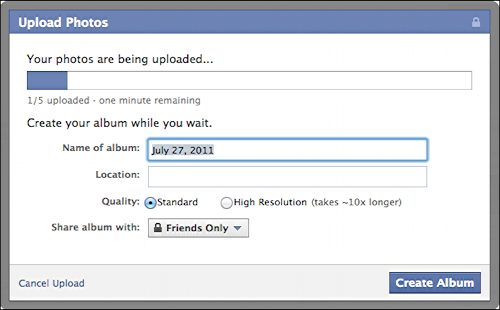
\includegraphics[width=5cm]{img-presentation/facebook-upload-photo-computer-6}
    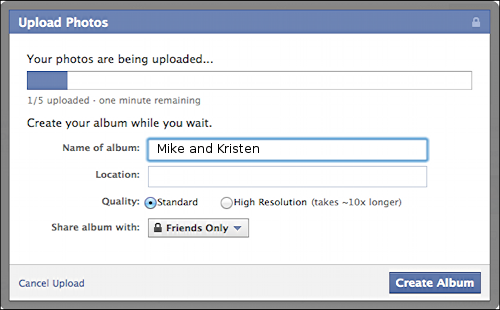
\includegraphics[width=5cm]{img-presentation/fb-upload}
};}
\uncover<2-6>{\node at (1.75,-3.75) {
    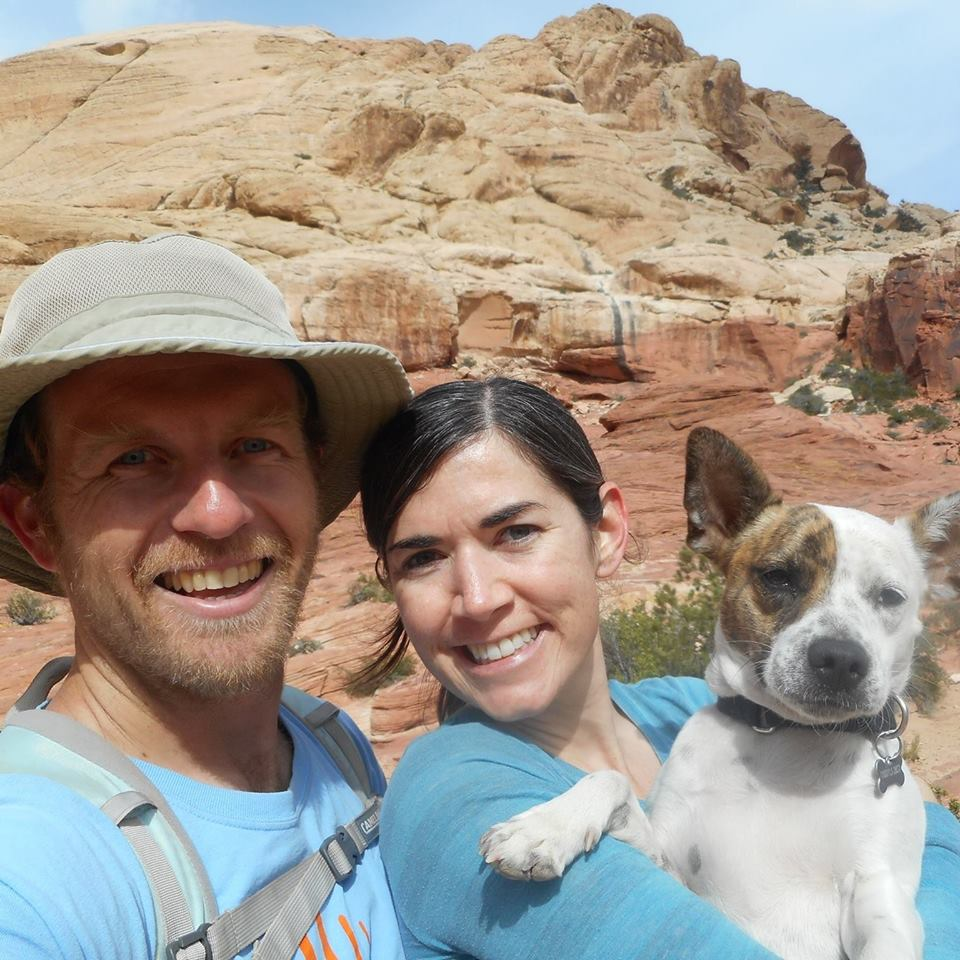
\includegraphics[width=3cm]{img-presentation/dog}
};}
\uncover<4-6>{\node at (5,-4.25) {
    %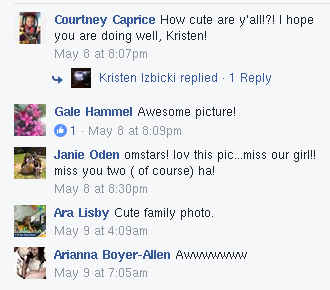
\includegraphics[width=3cm]{img-presentation/dog-message}
    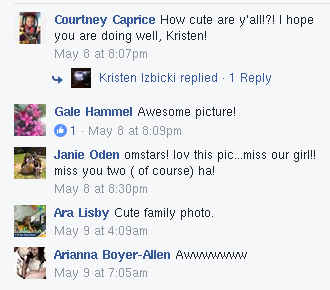
\includegraphics[width=4cm]{img-presentation/dog-message}
};}
\uncover<5-6>{\node at (3.5,-6.5) {
    
\includegraphics[width=3cm]{img-presentation/fb-like}
};}
}

%%%%%%%%%%%%%%%%%%%%%%%%%%%%%%%%%%%%%%%%

\uncover<6-9>{
\node at (-4.35,-1.5) {
\includegraphics[width=0.2cm]{img-presentation/dot}};
\node[text width=10cm] at (1,-1.5) {
    machine learning algorithms use this data to solve problems
};
\uncover<7-9>{
\node[text width=10cm] at (1,-2.0) {like identifying people in images
{\uncover<8-9>{and displaying profitable ads}}};
}

\uncover<7-8>{
\node at (-2,-5) {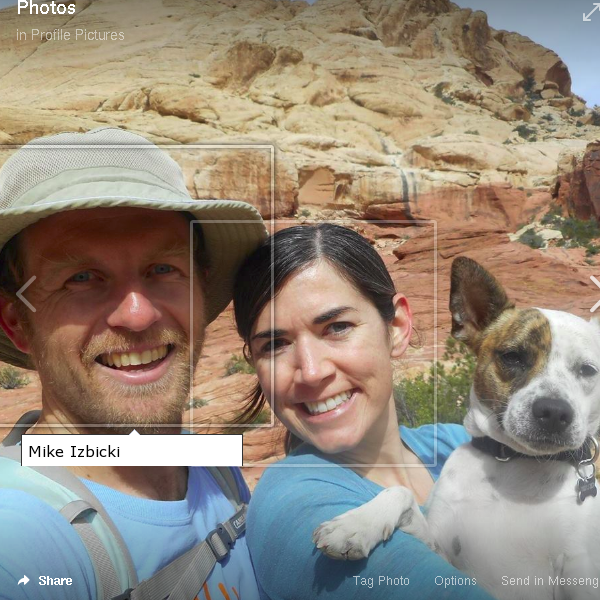
\includegraphics[width=5cm] {img-presentation/fb-faces2}};
}
\uncover<8>{\node at (4,-5) {
    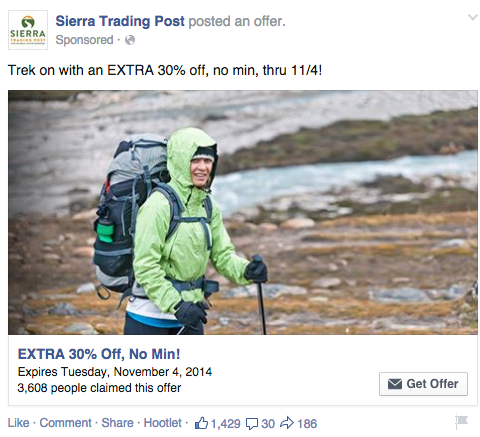
\includegraphics[width=5cm] {img-presentation/fb-ad-hiking}
};}
}

%%%%%%%%%%%%%%%%%%%%%%%%%%%%%%%%%%%%%%%%

\uncover<9> {
\node[text width=12cm] at (1,-2.6) {\textbf{Challenge:} we need new, faster algorithms to process this data};
%\node[text width=6cm] at (-2,-3.1) {Facebook has ``an estimated hundreds of thousands'' of computers};
%\node at (4,-5) {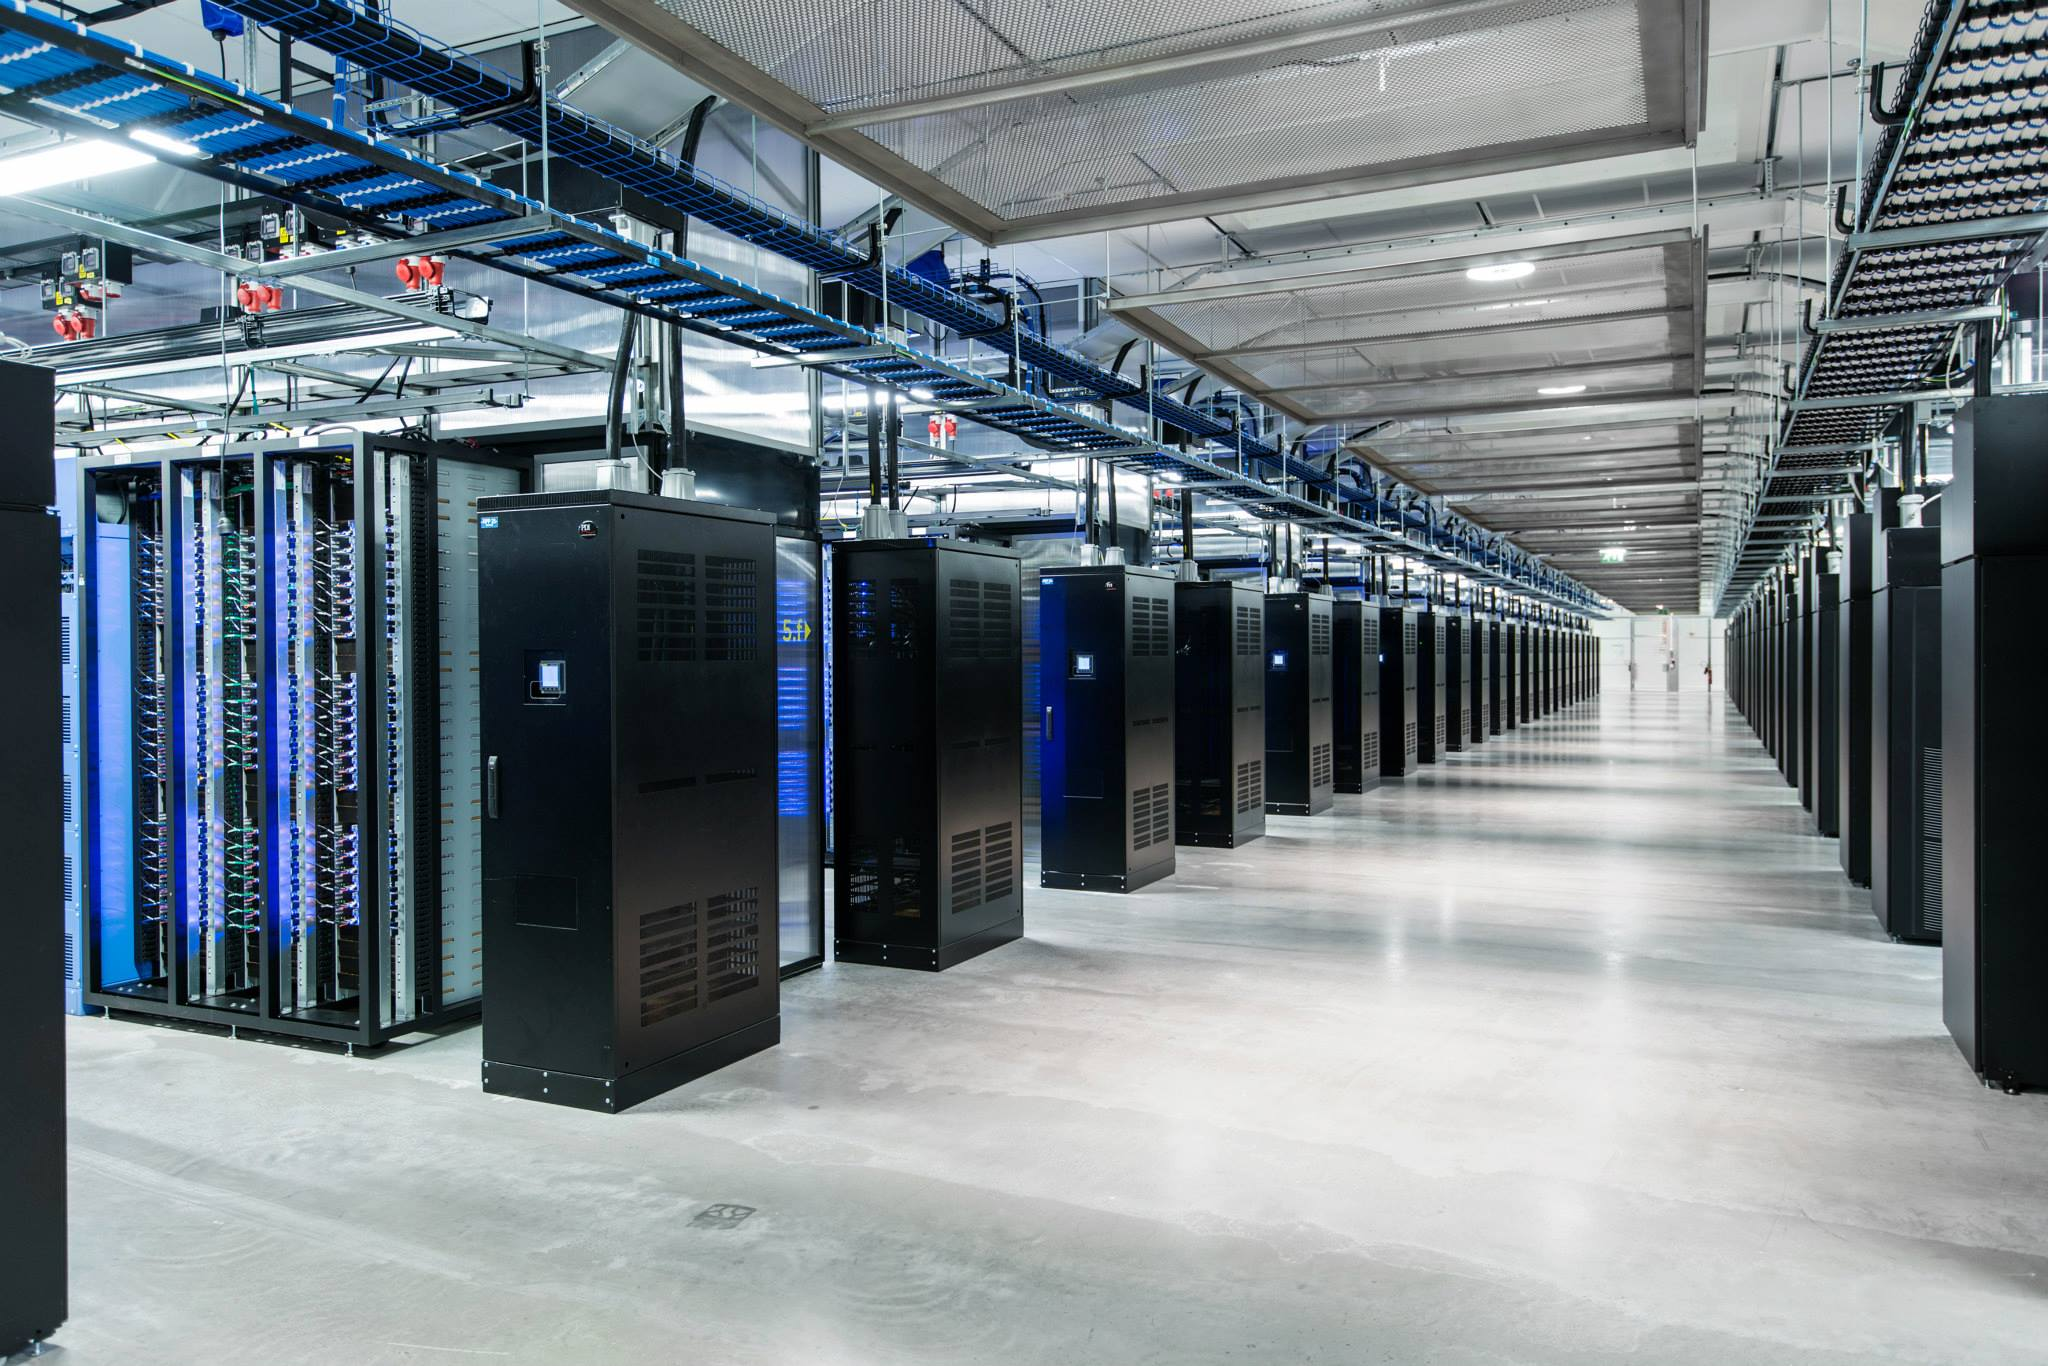
\includegraphics[width=6cm]{img-presentation/facebook_10969}};
}

%%%%%%%%%%%%%%%%%%%%%%%%%%%%%%%%%%%%%%%%

\end{tikzpicture}

%This data is stored on ``hundreds of thousands'' of computers
%
%(Facebook Datacenter FAQ)

\end{frame}

%%%%%%%%%%%%%%%%%%%%%%%%%%%%%%%%%%%%%%%%%%%%%%%%%%%%%%%%%%%%%%%%%%%%%%%%%%%%%%%%

\begin{frame}{Many organizations need faster machine learning}

\begin{itemize}
\item 
computer companies

\vspace{0.05in}
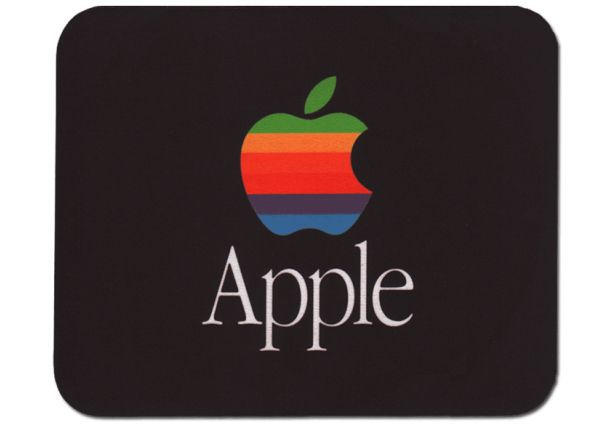
\includegraphics[height=1cm]{img-presentation/apple}~~~

\includegraphics[height=1cm]{img-presentation/ms}~~~

\includegraphics[height=1cm]{img-presentation/google}

\vspace{0.05in}

\includegraphics[height=1cm]{img-presentation/linkedin}~~~

\includegraphics[height=1cm]{img-presentation/yahoo}

\pause
\vspace{0.1in}
\item
traditional engineering

\vspace{0.05in}

\includegraphics[height=1cm]{img-presentation/pfizer}~~~

\includegraphics[height=1cm]{img-presentation/gm}

\pause
\vspace{0.1in}
\item 
pure scientific research

\vspace{0.05in}

\includegraphics[height=1cm]{img-presentation/nasa}~~~
%
\includegraphics[height=1cm]{img-presentation/nsf}~~~

\includegraphics[height=1cm]{img-presentation/cern}~~~

\includegraphics[height=1cm]{img-presentation/nih}

\end{itemize}

\end{frame}

%%%%%%%%%%%%%%%%%%%%%%%%%%%%%%%%%%%%%%%%%%%%%%%%%%%%%%%%%%%%%%%%%%%%%%%%%%%%%%%%

\begin{frame}{My research}
\textbf{Goal:} 
%Goal:
%\begin{itemize}
%\item
generic techniques that make machine learning faster for everyone

%for all these organizations
%\end{itemize}

\pause
\vspace{0.15in}
Examples
\begin{itemize}
\item
ad-click data from the Tencent search engine

(improve ad revenue for a given computational budget)

\vspace{-1.5cm}
\begin{tikzpicture}
\node at (0,0) {};
\node at (10,0) {
\includegraphics[width=2cm]{img-presentation/tencent}};
\end{tikzpicture}
%\vspace{-1cm}

\pause
\item
protein data bank

(first analysis of approximately 100,000 human 

proteins using random walk graph kernels)

\vspace{-1.5cm}
\begin{tikzpicture}
\node at (0,0) {};
\node at (9.5,0) {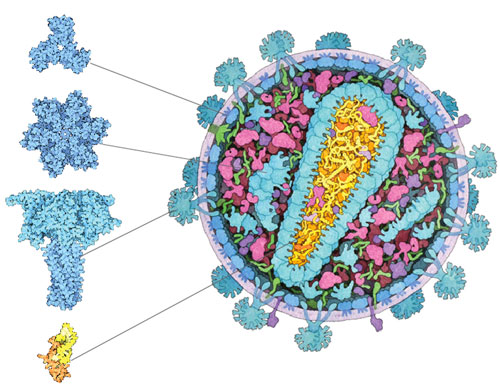
\includegraphics[width=2.5cm]{img-presentation/pdb}};
\end{tikzpicture}

\pause
\vspace{-0.4cm}
\item
Flickr creative commons images

(find patterns in 1.5 million images on a single machine)
\end{itemize}

\vspace{-0.8cm}
\begin{tikzpicture}
\node at (0,0) {};
\node at (11,0) {
\includegraphics[width=1.3cm]{img-presentation/flikr}};
\end{tikzpicture}

\pause
\vspace{-0.15in}
Main contributions are \textbf{theoretical} and \textbf{more general}
\end{frame}
